\chapter{Disk Management and Disk Scheduling}

\section{Introduction}

Storage systems are critical components of modern operating systems. Efficient disk management directly affects application performance, database throughput, file system responsiveness, and overall system efficiency.

This chapter covers traditional magnetic disks, modern SSDs, disk scheduling algorithms, RAID technologies, and interview-focused numerical problem solving.

\section{Learning Objectives}

After completing this chapter, you should be able to:

\begin{itemize}
\item Understand magnetic disk organization.
\item Explain SSD architecture.
\item Calculate seek times and head movements.
\item Solve disk scheduling numericals.
\item Compare scheduling algorithms.
\item Understand RAID levels and fault tolerance.
\item Explain wear leveling and TRIM.
\item Answer common interview questions.
\end{itemize}

%====================================================
\section{Magnetic Disks Overview}
%====================================================

\subsection{Definition}

A magnetic disk stores data using magnetized surfaces on rotating platters.

\subsection{Components}

\begin{itemize}
\item Platters
\item Spindle
\item Read/Write Heads
\item Disk Controller
\end{itemize}

\subsection{Characteristics}

\begin{itemize}
\item Mechanical movement
\item Large storage capacity
\item Low cost per GB
\item Higher latency than SSDs
\end{itemize}

\section{SSD Overview}

\subsection{Definition}

Solid State Drives (SSDs) store data in flash memory rather than magnetic platters.

\subsection{Characteristics}

\begin{itemize}
\item No moving parts
\item Lower latency
\item Faster reads
\item Lower power consumption
\item More expensive per GB
\end{itemize}

\subsection{Advantages over HDDs}

\begin{itemize}
\item Faster boot times
\item Better random access
\item Silent operation
\item Shock resistance
\end{itemize}

%====================================================
\section{Disk Structure}
%====================================================

Magnetic disks are organized into:

\begin{itemize}
\item Platters
\item Tracks
\item Sectors
\item Cylinders
\end{itemize}

\begin{figure}[h]
\centering
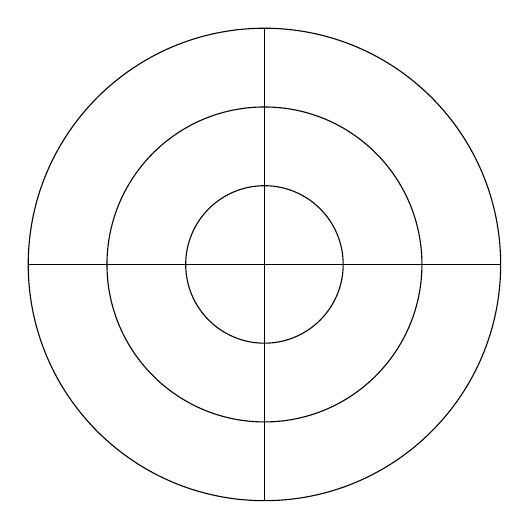
\begin{tikzpicture}
\draw (0,0) circle (3cm);
\draw (0,0) circle (2cm);
\draw (0,0) circle (1cm);

\draw (0,0)--(3,0);
\draw (0,0)--(-3,0);
\draw (0,0)--(0,3);
\draw (0,0)--(0,-3);
\end{tikzpicture}
\caption{Disk Structure}
\end{figure}

%====================================================
\section{Tracks}
%====================================================

\subsection{Definition}

A track is a circular path on the disk surface where data is recorded.

\subsection{Characteristics}

\begin{itemize}
\item Concentric circles
\item Divided into sectors
\item Multiple tracks per platter
\end{itemize}

\section{Sectors}

\subsection{Definition}

A sector is the smallest physical storage unit on a disk.

\subsection{Typical Sizes}

\begin{itemize}
\item 512 Bytes
\item 4 KB (Advanced Format)
\end{itemize}

\section{Cylinders}

\subsection{Definition}

A cylinder consists of all tracks located at the same radius across multiple platters.

\begin{figure}[h]
\centering
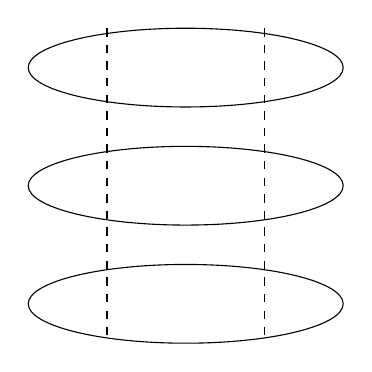
\begin{tikzpicture}

\draw (0,0) ellipse (2 and 0.5);
\draw (0,-1.5) ellipse (2 and 0.5);
\draw (0,-3) ellipse (2 and 0.5);

\draw[dashed] (-1,0.5)--(-1,-3.5);
\draw[dashed] (1,0.5)--(1,-3.5);

\end{tikzpicture}
\caption{Cylinder Across Platters}
\end{figure}

\section{Seek Time}

\subsection{Definition}

Time required to move the read/write head to the target track.

\subsection{Formula}

\[
Seek\ Time \propto Distance\ Moved
\]

\subsection{Example}

Current Track:

\[
50
\]

Target Track:

\[
120
\]

Head Movement:

\[
|120-50|=70
\]

tracks.

\section{Rotational Latency}

\subsection{Definition}

Time waiting for the desired sector to rotate under the read/write head.

\subsection{Average Rotational Latency}

\[
\frac{1}{2}\times Rotation\ Time
\]

\subsection{Example}

7200 RPM disk:

\[
Rotation\ Time=\frac{60}{7200}
\]

\[
=8.33ms
\]

Average Latency:

\[
4.17ms
\]

\section{Transfer Time}

\subsection{Definition}

Time required to transfer data once the correct sector reaches the head.

\subsection{Factors}

\begin{itemize}
\item Data Size
\item Disk Speed
\item Controller Speed
\end{itemize}

\section{Disk Access Time}

\[
Disk\ Access\ Time=
Seek\ Time+
Rotational\ Latency+
Transfer\ Time
\]

%====================================================
\section{Disk Scheduling Concepts}
%====================================================

Disk scheduling determines the order in which pending disk requests are serviced.

\subsection{Goals}

\begin{itemize}
\item Reduce seek time
\item Improve throughput
\item Reduce waiting time
\item Improve response time
\end{itemize}

\subsection{Example Queue}

\[
98,183,37,122,14,124,65,67
\]

Initial Head:

\[
53
\]

This queue will be used throughout the chapter.

%====================================================
\section{FCFS (First Come First Serve)}
%====================================================

\subsection{Working}

Requests are serviced in arrival order.

\subsection{Sequence}

\[
53 \rightarrow 98 \rightarrow 183 \rightarrow 37
\]

\[
\rightarrow 122 \rightarrow 14 \rightarrow 124
\]

\[
\rightarrow 65 \rightarrow 67
\]

\subsection{Head Movement}

\[
45+85+146+85+108+110+59+2
\]

\[
=640
\]

tracks.

\subsection{Advantages}

\begin{itemize}
\item Fair
\item Simple
\end{itemize}

\subsection{Disadvantages}

\begin{itemize}
\item Poor performance
\item High seek time
\end{itemize}

%====================================================
\section{SSTF (Shortest Seek Time First)}
%====================================================

\subsection{Working}

Choose request closest to current head.

\subsection{Sequence}

\[
53 \rightarrow 65 \rightarrow 67 \rightarrow 37
\]

\[
\rightarrow 14 \rightarrow 98 \rightarrow 122
\]

\[
\rightarrow 124 \rightarrow 183
\]

\subsection{Head Movement}

\[
12+2+30+23+84+24+2+59
\]

\[
=236
\]

tracks.

\subsection{Advantages}

\begin{itemize}
\item Better throughput
\item Lower seek time
\end{itemize}

\subsection{Disadvantages}

\begin{itemize}
\item Starvation possible
\end{itemize}

%====================================================
\section{SCAN Algorithm}
%====================================================

\subsection{Working}

Disk arm moves in one direction servicing requests.

At end, reverses direction.

\subsection{Nickname}

Elevator Algorithm.

\subsection{Example}

Direction:

\[
\rightarrow
\]

Sequence:

\[
53 \rightarrow 65 \rightarrow 67 \rightarrow 98
\]

\[
\rightarrow 122 \rightarrow 124 \rightarrow 183
\]

Then reverse.

\subsection{Advantages}

\begin{itemize}
\item Good throughput
\item Fair
\end{itemize}

\subsection{Disadvantages}

\begin{itemize}
\item End tracks may wait longer
\end{itemize}

%====================================================
\section{CSCAN Algorithm}
%====================================================

\subsection{Working}

Head moves only in one direction.

After reaching end:

\begin{itemize}
\item Returns immediately to beginning.
\item Continues scanning.
\end{itemize}

\subsection{Advantages}

\begin{itemize}
\item Uniform waiting times
\end{itemize}

\subsection{Disadvantages}

\begin{itemize}
\item Additional movement
\end{itemize}

%====================================================
\section{LOOK Algorithm}
%====================================================

\subsection{Working}

Like SCAN but reverses at last request.

Does not move to physical disk end.

\subsection{Advantages}

\begin{itemize}
\item Less movement
\item Better efficiency
\end{itemize}

\subsection{Disadvantages}

\begin{itemize}
\item Slightly more complex
\end{itemize}

%====================================================
\section{CLOOK Algorithm}
%====================================================

\subsection{Working}

Like CSCAN but jumps from last request to first request.

\subsection{Advantages}

\begin{itemize}
\item Reduced unnecessary movement
\end{itemize}

\subsection{Disadvantages}

\begin{itemize}
\item More bookkeeping
\end{itemize}

%====================================================
\section{Scheduling Diagram}
%====================================================

\begin{figure}[h]
\centering
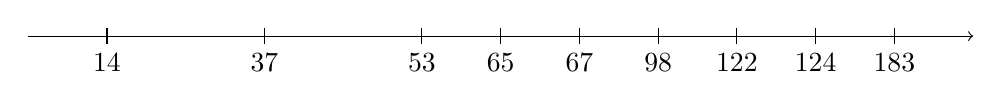
\begin{tikzpicture}

\draw[->] (0,0)--(12,0);

\foreach \x/\t in {1/14,3/37,5/53,6/65,7/67,8/98,9/122,10/124,11/183}
{
\draw (\x,0.1)--(\x,-0.1);
\node[below] at (\x,-0.1) {\t};
}

\end{tikzpicture}
\caption{Disk Request Positions}
\end{figure}

%====================================================
\section{RAID Levels}
%====================================================

\subsection{Definition}

RAID (Redundant Array of Independent Disks) combines multiple disks to improve:

\begin{itemize}
\item Performance
\item Reliability
\item Fault Tolerance
\end{itemize}

\section{RAID 0}

\subsection{Concept}

Striping only.

\begin{figure}[h]
\centering
\begin{tabular}{|c|c|}
\hline
Disk 1 & Disk 2 \\
\hline
A1 & A2 \\
B1 & B2 \\
C1 & C2 \\
\hline
\end{tabular}
\caption{RAID 0}
\end{figure}

\subsection{Advantages}

\begin{itemize}
\item Highest performance
\end{itemize}

\subsection{Disadvantages}

\begin{itemize}
\item No fault tolerance
\end{itemize}

%====================================================
\section{RAID 1}
%====================================================

\subsection{Concept}

Mirroring.

\begin{figure}[h]
\centering
\begin{tabular}{|c|c|}
\hline
Disk 1 & Disk 2 \\
\hline
A & A \\
B & B \\
C & C \\
\hline
\end{tabular}
\caption{RAID 1}
\end{figure}

\subsection{Advantages}

\begin{itemize}
\item High reliability
\end{itemize}

\subsection{Disadvantages}

\begin{itemize}
\item 50\% storage efficiency
\end{itemize}

%====================================================
\section{RAID 5}
%====================================================

\subsection{Concept}

Striping with distributed parity.

\subsection{Characteristics}

\begin{itemize}
\item Minimum 3 disks
\item Survives one disk failure
\end{itemize}

\subsection{Advantages}

\begin{itemize}
\item Good balance
\end{itemize}

\subsection{Disadvantages}

\begin{itemize}
\item Write penalty
\end{itemize}

%====================================================
\section{RAID 6}
%====================================================

\subsection{Concept}

Dual distributed parity.

\subsection{Characteristics}

\begin{itemize}
\item Survives two disk failures
\end{itemize}

\subsection{Advantages}

\begin{itemize}
\item Higher reliability
\end{itemize}

\subsection{Disadvantages}

\begin{itemize}
\item More parity overhead
\end{itemize}

%====================================================
\section{RAID 10}
%====================================================

\subsection{Concept}

Mirroring + Striping.

\[
RAID1 + RAID0
\]

\subsection{Advantages}

\begin{itemize}
\item Excellent performance
\item Excellent reliability
\end{itemize}

\subsection{Disadvantages}

\begin{itemize}
\item Expensive
\end{itemize}

%====================================================
\section{RAID Comparison}
%====================================================

\begin{table}[h]
\centering
\small
\begin{tabular}{|c|c|c|c|}
\hline
RAID & Performance & Fault Tolerance & Efficiency \\
\hline
0 & Excellent & None & 100\% \\
1 & Good & High & 50\% \\
5 & Good & 1 Disk & High \\
6 & Moderate & 2 Disks & Moderate \\
10 & Excellent & High & 50\% \\
\hline
\end{tabular}
\caption{RAID Comparison}
\end{table}

%====================================================
\section{SSD Internals}
%====================================================

SSD consists of:

\begin{itemize}
\item NAND Flash
\item Controller
\item DRAM Cache
\item Firmware
\end{itemize}

\subsection{Organization}

\[
Page \rightarrow Block \rightarrow Chip
\]

\subsection{Characteristics}

\begin{itemize}
\item Reads fast
\item Writes more expensive
\item Erase-before-write
\end{itemize}

%====================================================
\section{Wear Leveling}
%====================================================

\subsection{Problem}

Flash cells have limited write cycles.

\subsection{Solution}

Wear leveling distributes writes evenly.

\subsection{Goal}

Prevent premature failure.

\subsection{Types}

\begin{itemize}
\item Dynamic Wear Leveling
\item Static Wear Leveling
\end{itemize}

%====================================================
\section{TRIM}
%====================================================

\subsection{Definition}

TRIM informs SSD which blocks are no longer needed.

\subsection{Benefits}

\begin{itemize}
\item Faster writes
\item Better garbage collection
\item Longer SSD lifespan
\end{itemize}

\subsection{Linux Example}

\begin{verbatim}
fstrim -v /
\end{verbatim}

%====================================================
\section{Solved Numerical Example}
%====================================================

Requests:

\[
98,183,37,122,14,124,65,67
\]

Head:

\[
53
\]

Using SSTF:

\[
53 \rightarrow 65 \rightarrow 67 \rightarrow 37
\]

\[
\rightarrow 14 \rightarrow 98 \rightarrow 122
\]

\[
\rightarrow 124 \rightarrow 183
\]

Total Movement:

\[
236
\]

tracks.

%====================================================
\section{Interview Tips}
%====================================================

\begin{itemize}
\item SSTF minimizes immediate seek time.
\item SCAN is called Elevator Algorithm.
\item LOOK avoids unnecessary end movement.
\item RAID 0 provides performance only.
\item RAID 1 provides mirroring.
\item RAID 5 survives one failure.
\item RAID 6 survives two failures.
\item RAID 10 combines speed and redundancy.
\item SSDs do not require traditional disk scheduling.
\item Wear leveling is a common interview topic.
\end{itemize}

%====================================================
\section{Key Takeaways}
%====================================================

\begin{itemize}
\item Disk performance depends on seek time, latency, and transfer time.
\item Disk scheduling reduces head movement.
\item SSTF improves over FCFS.
\item SCAN and LOOK are commonly discussed algorithms.
\item RAID improves reliability and performance.
\item SSDs differ fundamentally from magnetic disks.
\item Wear leveling extends SSD life.
\item TRIM improves SSD performance.
\end{itemize}

%====================================================
\section{25 Interview Questions with Answers}
%====================================================

\begin{enumerate}
\item What is seek time?\\
Answer: Time to move disk head.

\item What is rotational latency?\\
Answer: Waiting for sector rotation.

\item What is transfer time?\\
Answer: Time to transfer data.

\item What is FCFS?\\
Answer: Arrival-order scheduling.

\item What is SSTF?\\
Answer: Closest request first.

\item SSTF drawback?\\
Answer: Starvation.

\item SCAN nickname?\\
Answer: Elevator Algorithm.

\item What is CSCAN?\\
Answer: Circular SCAN.

\item What is LOOK?\\
Answer: SCAN without going to disk end.

\item What is CLOOK?\\
Answer: Circular LOOK.

\item Define RAID.\\
Answer: Redundant Array of Independent Disks.

\item RAID 0 provides?\\
Answer: Striping.

\item RAID 1 provides?\\
Answer: Mirroring.

\item RAID 5 survives?\\
Answer: One disk failure.

\item RAID 6 survives?\\
Answer: Two disk failures.

\item RAID 10 combines?\\
Answer: Mirroring and Striping.

\item SSD stores data using?\\
Answer: Flash Memory.

\item SSD has moving parts?\\
Answer: No.

\item What is wear leveling?\\
Answer: Even write distribution.

\item Why TRIM?\\
Answer: Identify unused blocks.

\item What is a track?\\
Answer: Circular recording path.

\item What is a sector?\\
Answer: Smallest physical unit.

\item What is a cylinder?\\
Answer: Same-radius tracks.

\item Best FCFS advantage?\\
Answer: Simplicity.

\item SSD scheduling needed?\\
Answer: Generally less important.
\end{enumerate}

%====================================================
\section{25 MCQs with Answers}
%====================================================

\begin{enumerate}
\item Smallest disk storage unit:
Answer: Sector

\item Circular storage path:
Answer: Track

\item Same-radius tracks:
Answer: Cylinder

\item FCFS stands for:
Answer: First Come First Serve

\item SSTF stands for:
Answer: Shortest Seek Time First

\item Elevator algorithm:
Answer: SCAN

\item Circular SCAN:
Answer: CSCAN

\item LOOK is improvement over:
Answer: SCAN

\item RAID 0 uses:
Answer: Striping

\item RAID 1 uses:
Answer: Mirroring

\item RAID 5 tolerates:
Answer: One Failure

\item RAID 6 tolerates:
Answer: Two Failures

\item RAID 10 combines:
Answer: RAID 0 and RAID 1

\item SSD uses:
Answer: NAND Flash

\item SSD moving parts:
Answer: None

\item Wear leveling improves:
Answer: Lifespan

\item TRIM improves:
Answer: SSD Performance

\item SSTF may cause:
Answer: Starvation

\item SCAN is:
Answer: Fairer than SSTF

\item FCFS is:
Answer: Simple

\item Average latency depends on:
Answer: Rotation Speed

\item Seek time depends on:
Answer: Head Movement

\item SSD latency compared to HDD:
Answer: Lower

\item RAID improves:
Answer: Reliability

\item Disk scheduling mainly reduces:
Answer: Seek Time
\end{enumerate}

%====================================================
\section{Revision Notes}
%====================================================

\begin{itemize}
\item Disk access time = Seek + Latency + Transfer.
\item SSTF selects nearest request.
\item SCAN = Elevator Algorithm.
\item LOOK avoids unnecessary movement.
\item RAID 0 = Striping.
\item RAID 1 = Mirroring.
\item RAID 5 = Single parity.
\item RAID 6 = Dual parity.
\item RAID 10 = Mirroring + Striping.
\item SSDs use flash memory.
\item Wear leveling extends SSD lifespan.
\item TRIM improves SSD efficiency.
\end{itemize}

%====================================================
\section{Cheat Sheet}
%====================================================

\begin{center}
\begin{tabular}{|p{5cm}|p{8cm}|}
\hline
Track & Circular Path \\
\hline
Sector & Smallest Physical Unit \\
\hline
Cylinder & Same Radius Tracks \\
\hline
Seek Time & Head Movement Time \\
\hline
Rotational Latency & Rotation Wait Time \\
\hline
Transfer Time & Data Transfer Time \\
\hline
FCFS & Arrival Order \\
\hline
SSTF & Closest Request \\
\hline
SCAN & Elevator Algorithm \\
\hline
CSCAN & Circular SCAN \\
\hline
LOOK & Optimized SCAN \\
\hline
CLOOK & Optimized CSCAN \\
\hline
RAID 0 & Striping \\
\hline
RAID 1 & Mirroring \\
\hline
RAID 5 & Single Parity \\
\hline
RAID 6 & Dual Parity \\
\hline
RAID 10 & Mirroring + Striping \\
\hline
SSD & Flash Storage \\
\hline
Wear Leveling & Even Writes \\
\hline
TRIM & Free Block Notification \\
\hline
\end{tabular}
\end{center}